\section{Experiments and Discussion}
\label{sec:Experiment}

In this chapter, we conduct experiments to evaluate our methods proposed
in \ref{sec:ClassificationMethod1} and \ref{sec:ClassificationMethod2},
and present the results obtained from them.  In addition, we discuss our
methods based on the results.

\subsection{Data Set}
\label{subsec:Data Set}

We collected the data set from the real Twitter data by using Twitter
API.

We first randomly selected 1,000 Twitter users whose timezone is Japan.
At this time, we omitted users followed from nobody or posting
no tweet in order to select only active users.  Then, we divided them in
two sets equally, i.e., each of which include 500 users.

Second, we had 6 experienced Twitter users as participants, all of whom
are male graduate students in engineering, from 23 to 25 years old.  We
assigned each set to 3 participants, and we asked each participant to
determine one of the following categories each user in the assigned set
is supposed to be in:

\begin{description}
\item[(i)] the user publishes information to the wide public,
\item[(ii)] the user publishes information to some specific topics,
\item[(iii)] the user publishes information to a specific group of users, and
\item[(iv)] the user publishes information (ii) on some specific topics
           (iii) to a specific group of users.
\end{description}

\noindent{These categories correspond to the category ``target
specificity is high'', (1), (2), and (3) in Figure~\ref{fig:Flow}
respectively.}

Then, we selected users whose category at least 2 out of 3 participants
coincide with, and as a result, we were able to collect 93, 320, 375,
and 30 users in the category (i), (ii), (iii), and (iv) respectively.  We randomly
selected 90 users from the category (i), and 30 users from each category
of (ii), (iii), and (iv).  We collected these 180 users in total, and we
used them as the data set.  Table~\ref{table:breakdown} shows the
breakdown of the data set: the average and the standard deviation of numbers of
followers, followees, and tweets in each category.

\begin{table}[t]
\caption{Breakdown of data set: average and standard deviation of
 numbers of followers, followees, and tweets in each category shown in
 the format of \emph{Average\,(SD)} \label{table:breakdown}}
\begin{center}
\begin{tabular}{@{}cccc@{}}
\toprule
\makebox[6em]{{\bf category}} & \makebox[8em]{{\bf follower}} &
 \makebox[8em]{{\bf followee}} & \makebox[8em]{{\bf tweet}} \\
 \cmidrule(lr){1-1}\cmidrule(lr){2-4}
 (i) & 475,679\,(535,894) & 11,274\,(37,906) & 9,763\,(14,607) \\
 (ii) & 58,142\,(171,784) & 3,353\,(7,218) & 9,992\,(23,572) \\
 (iii) & 573\,(1,389) & 598\,(1,545) & 8,829\,(29,505) \\
 (iv) & 82,942\,(262,161) & 1,568\,(3,594) & 5,677\,(6,600) \\
\bottomrule
\end{tabular}
\end{center}
\end{table}

Then, for each user, we collected at most 1,000 followers, their
profiles and local information, and at most 1,000 followees of them.
When collecting this data, we removed terms and
followees whose local rate is 0.01 or below to reduce calculation costs.
In addition, we also removed stop words from profiles and local
information. Especially in this experiments, we included
Twitter original words, e.g., tweet, follow, and so on, in the stop word
list.  We used this data in order to evaluate our methods.

\subsection{Experimental Settings and Libraries}
\label{subsec:Settings}

First, we conducted the experiments evaluating the method of classifying
users based on target specificity of their information
publishing mentioned in \ref{sec:ClassificationMethod1}.  We used 90
users in the category (i) as target users, and 90 users
in the categories (ii), (iii), and (iv) as non target users.
We first computed $\mathit{SpecificityScore}_{{\mathit{term}}}(u)$ and
$\mathit{SpecificityScore}_{{\mathit{followee}}}(u)$ for each user $u$
using a couple of models, i.e., the probablistic model and the
subtracting model mentioned in \ref{subsec:Scoring}, and computed the
accuracy of the classification of
target users and non target users using each attribute separately.  In
regard to the probablistic model, we take 0.01, 0.03, 0.05 for $\gamma$,
the threshold which cuts down the case that a local rate is very small,
and compared them.  When
computing $\mathit{SpecificityScore}_{{\mathit{followee}}}(u)$, we
assumed that the rate of active users in Twitter is 0.01.

Next, we computed $\mathit{TargetSpecificity}(u)$
based on the above scores using a couple of baselines and four types of
proposed methods.  A couple of baselines are as follows:

\noindent{{\bf follower}: numbers of followers arranged in the descending order,
and}

\noindent{{\bf SVM}: a binary SVM with the features of the max rate of common
           terms in profiles and location information and common
           followees in followers.}

\noindent{For types of proposed methods are the average and the maximum of the
above two scores and a binary classifier with the features of two scores
adopting SVM and the decision tree mentioned in \ref{subsec:Final
Classification}.}

Then, we
determined a threshold $\delta$ which can classify target users and
non target users accurately the most, and evaluated the classification
results with $\delta$.

Second, we conducted the experiments evaluating the method of determining
why target specificity of the users is high in regard to target
users mentioned in \ref{sec:ClassificationMethod2}.  We extracted 30 users
from each category of (ii), (iii), and (iv), and used 90 users
in total.  We first extracted features mentioned in
\ref{subsec:Features} from the user, which are normalized to a
value between $0$ and $1$.  Then, based on these features, we
constructed two types of classification approaches: a 3-class
classifier and
2 binary classifiers mentioned in \ref{subsec:Architecture}, which
classify users into three categories:
(ii), (iii), and (iv), and evaluated the classification results using
3-fold cross validation.  We used two learning algorithms: SVM and the
decision tree as a classifier, and compared them.  For SVM, we used
LIBSVM\footnote{\url{http://www.csie.ntu.edu.tw/~cjlin/libsvm/}}, which
is a popular SVM library, with the Gaussian kernel, which using
one-against-one method for multiclass classification.  For the decision
tree, we used scikit-learn
\footnote{\url{http://scikit-learn.org/stable/modules/tree.html}}, which
is a Python module for machine learning.

We used twpro search API\footnote{\url{http://twpro.jp/doc/api/search}}
in order to get a number of users having a certain term in their
profiles.  We also used
MeCab\footnote{\url{http://mecab.sourceforge.net/}} for morphological
analysis of Japanese sentences in profiles, local information, and
tweets of users.  Furthermore, we used
gensim\footnote{\url{http://radimrehurek.com/gensim/}} for using Latent
Dirichlet Allocation (LDA).

\subsection{Results and Evaluation of Classifying Users Based on Target
  Specificity}
\label{subsec:Results of Method1}

In this subchapter, we show the results of the experiments classifying
users based on target specificity of their information publishing.

We first show the accuracy of the classification of target users and
non target users using a couple of attributes measuring consistency,
i.e., common terms and common followers, separately.  We also used a
couple of models, i.e., the
probablistic model and the subtracting model, which compute
$\mathit{SubsetScore}(S_{F_uc})$.
The 3rd and 4th rows of Table~\ref{table:Classify
Target Users} show the accuracy of the classification using common
terms and common followees as attributes, respectively.  For each
attribute, a bold number shows when the accuracy becomes the highest.

\begin{table}[t]
\caption{Accuracy of the classification of target users and non target
 users using a couple of attributes measuring consistency separately
 \label{table:Classify Target Users}}
\begin{center}
\begin{tabular}{ccccc}
 \toprule
 {\bf attributes} & \multicolumn{3}{c}{{\bf Probablistic Model}} & {\bf
 Subtracting Model} \\
 & $\gamma = 0.01$ & $\gamma = 0.03$ & $\gamma = 0.05$ & \\
 \cmidrule(lr){1-1}\cmidrule(lr){2-4}\cmidrule(lr){5-5}
 common terms & {\bf 0.861} & 0.850 & 0,839 & 0.850 \\
 common followees & 0.828 & 0.828 & 0.817 & {\bf 0.833} \\
 \bottomrule
\end{tabular}
\end{center}
\end{table}

In each case of using common terms and common followees as attributes,
we achieved the highest accuracy when we used the probablistic model
with $\gamma = 0.01$ and the subtracting model respectively.  In regard
to the probablistic model, we can see that the smaller $\gamma$ is,
the higher the accuracy is.  This suggests that rare attributes
characterize target users though the covering rate of $S_{F_uc}$ to
$F_u$ is not high, and can contribute the classification of target users
and non target users.  But for both attributes, the difference between
the accuracy of the probablistic model and that of the subtracting
model is not so big.  So it is supposed that these two models are
about the same effect.

In addition, the accuracy using common terms as attributes is higher
than that using common followees regardless of models.  This suggests
that common terms in profiles and location information are more useful for
extracting consistency subsets than common followees.  This is supposed
to be because not only target users but also non target users sometimes
have common followees in their followers, though there is a little
possibility that non target users have common terms in their followers.
For example, a non target user publishing information about world news
sometimes have common followees publishing world news in
his followers.  But the global rate of such followers is usually
large, so there is no necessity to notice about them in most
cases.

{\footnotesize
\begin{figure}[t]
\begin{center}
\includegraphics[width=14cm]{images/histogram.eps}
 \caption{The histogram of specificity scores of each attribute on
 target users and non target users}
\label{fig:histogram}
\end{center}
\end{figure}
}

Now for each attribute, we use the model which is the highest accuracy,
i.e., the probablistic model with $\gamma=0.01$ for common terms and the
subtracting model for common
followees. Figure~\ref{fig:histogram} shows the histogram of specificity
scores of each attribute on target users and non target users.  In the
case of using common terms as attributes, specificity scores of most
non target users are very small, with the average 0.004.  On the other
hand, those of most target users are large, and even the average, 0.065,
is as same as the maximum score for non target users, i.e., 0.067.  A
similar trend is apparent in the case of using common followees as
attributes: even the median for target users, i.e., 0.050, is larger
than the maximum score for non target users, i.e., 0.043.

{\footnotesize
\begin{figure}[t]
\begin{center}
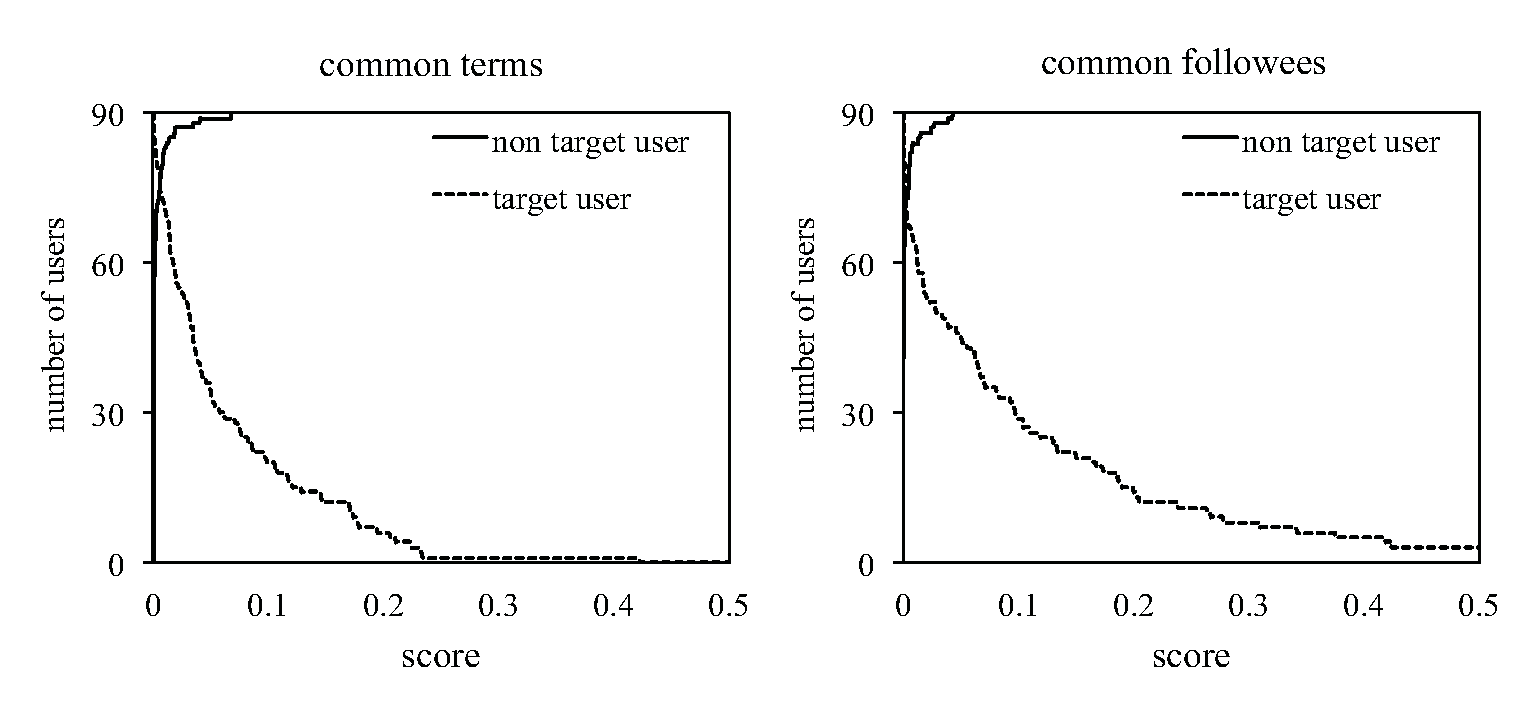
\includegraphics[width=14cm]{images/cumulativehistogram.eps}
 \caption{The cumulative histogram of specificity scores of each
 attribute on target users and non target users}
\label{fig:cumulativehistogram}
\end{center}
\end{figure}
}

{\footnotesize
\begin{figure}[t]
\begin{center}
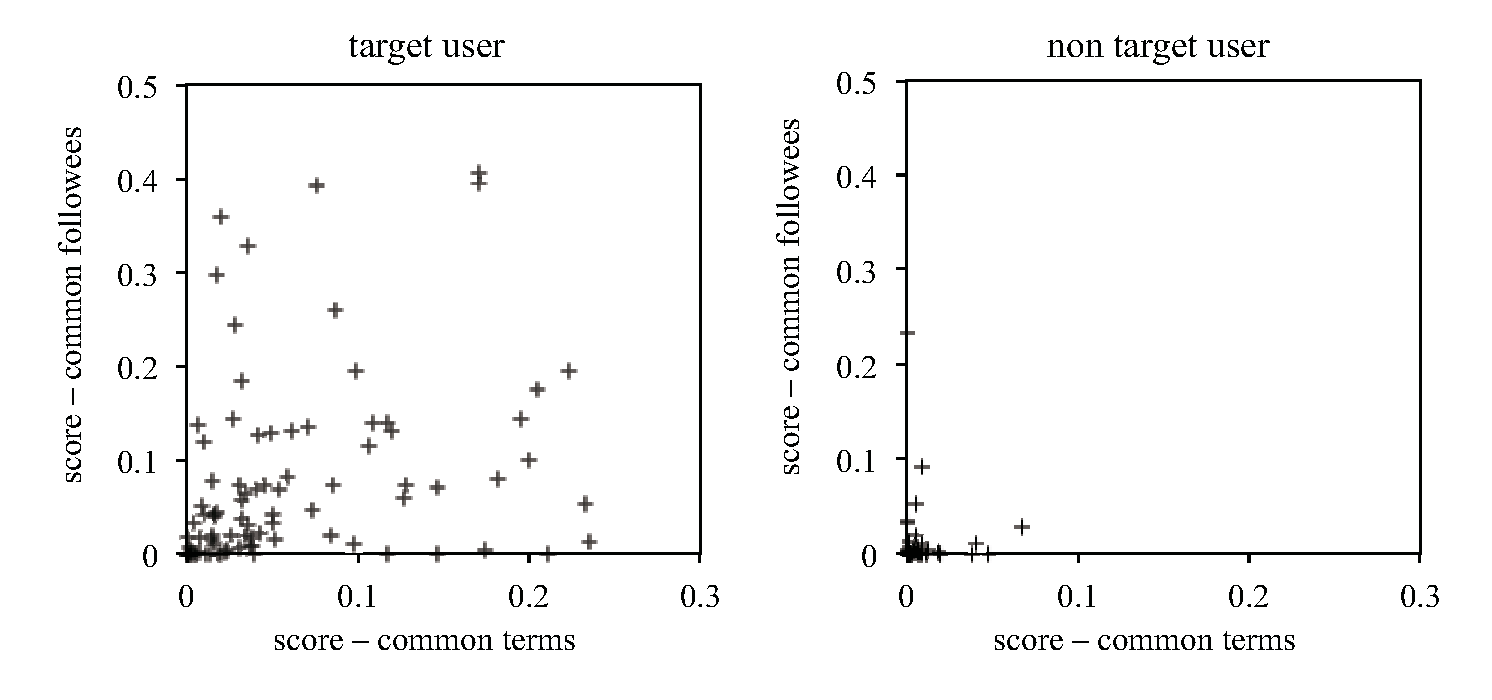
\includegraphics[width=14cm]{images/distribution.eps}
 \caption{A scatter diagram based on specificity scores of a couple of
 attributes, common terms and common followees, on target users and non
 target users}
\label{fig:distribution}
\end{center}
\end{figure}
}

Figure~\ref{fig:cumulativehistogram} shows the cumulative histogram of
specificity scores of each attribute on target users and non target
users.  More and more target users cumulate as scores become smaller,
and more and more non target users cumulate as scores become larger.
Therefore, the score on which the sum of numbers of target users and non
target users is the largest is the score which can classify target
users and non target users accurately the most, and we set this score
to the threshold $\delta$.  In the cases of using common terms and
common followees as attributes, we take $\delta$ for 0.009 and 0.012
respectively.

Next, we show the relationship between two attributes, i.e., common
terms and common followees.  Figure~\ref{fig:distribution} shows a
scatter diagram based on specificity scores of these two attributes on
target users and non target users.  On target users, points of scores of
these attributes are widely distributed and have weak positive
correlation, with the correlation coefficient 0.507.  That is, there is a
high possibility that the higher one score is, the higher the other
score is.  Of course, as shown in Figure~\ref{fig:distribution}, there
are some outliers, i.e., one score is high and the other score is low.
On the other hand, points of scores of these attributes concentrate on
the point $(0, 0)$ on no target users, and have no correlation, with the
correlation coefficient 0.232.

\begin{table}[t]
\caption{Accuracy of the final classification of target users and non
 target users \label{table:Final Accuracy}}
\begin{center}
\begin{tabular}{cccccc}
 \toprule
 \multicolumn{2}{c}{{\bf Baseline}} & \multicolumn{4}{c}{{\bf Proposed
 Method}} \\
 \makebox[4em]{follower} & \makebox[4em]{SVM} & \makebox[4em]{max} &
 \makebox[4em]{avg} & \makebox[4em]{SVM} & \makebox[5em]{decision
 tree} \\
 \cmidrule(lr){1-2}\cmidrule(lr){3-6}
 0.878 & 0.828 & 0.856 & 0.872 & {\bf 0.944} & 0.906 \\
 \bottomrule
\end{tabular}
\end{center}
\end{table}

Then, we show the accuracy of the final classification of target users
and non target users.  The 1st and 2nd columns of
Table~\ref{table:Final Accuracy} show the accuracy of a couple of
baselines: a follower method and a SVM method mentioned in
\ref{subsec:Settings}, respectively.  The accuracy
of the follower method achieved 0.878, which suggests that target
specificity is mainly related to a number of followers.  This
accuracy is quite high for a baseline, but notice that our final goal
is classifying outliers: target users who have many followers or non
target users who have a few followers, with high accuracy.  While the
accuracy of the SVM method was 0.828.

The following columns show the accuracy of four types of proposed
methods: the maximum and the average of scores of each attribute,
and a binary classifier with the features of these scores adopting
SVM and the decision tree, respectively.  The accuracy of the
maximum score was 0.856, which was lower than the accuracy using only
common terms as attributes as shown in Table~\ref{table:Classify Target
Users}, i.e., 0.861.  This suggests that some non
target users may have high scores in either attribute, and they are able
to become noises for the classification.  The accuracy of the average
score was 0.872, which was higher than the accuracy using common
terms or common followees separately as attributes, but lower than a follower
method, i.e., 0.878.  The accuracy of a binary classifier adopting SVM and the
decision tree achieved 0.944 and 0.906 respectively.  The former was the
highest accuracy of four types of proposed methods, and 0.66
point higher than the follower method.  This suggests that a binary classifier
adopting SVM is also able to classify users who is difficult to classify by
only a number of followers, i.e., target users who have many followers or non
target users who have a few followers with a certain degree of high accuracy.

\begin{table}[p]
\caption{Details of the results of a part of users
 \label{table:Details}}
\begin{center}
\scalebox{0.73}{
\begin{tabular}{cccccc}
 \toprule
 {\bf target user}  & {\bf term} \& {\bf followee} & $\mathit{local\,
 rate}$ & $\mathit{global\,rate}$ & $\mathit{SubsetScore}$ &
 $\mathit{SpecificityScore}$ \\ \midrule
 \multirow{6}{*}{@MCstaff\_Fukuoka} & Fukuoka & 0.563 & 0.047 & 0.390 & \\
 & music & 0.114 & 0.096 & 0.076 & 0.235 \\
 & Hakata & 0.095 & 0.003 & 0.076 & \\ \cmidrule(lr){2-6}
 & @fukuoka\_yokane & 0.069 & 0.023 & 0.046 &\\
 & @f\_sunpalace & 0.063 & 0.023 & 0.040 & 0.010 \\
 & @mbc\_o2\_eiji & 0.059 & 0.028 & 0.031 & \\ \midrule
 \multirow{6}{*}{@Jars0830} & Arashi & 0.439 & 0.039 & 0.304 & \\
 & participation & 0.190 & 0.026 & 0.131 & 0.233 \\
 & line & 0.130 & 0.045 & 0.090 & \\ \cmidrule(lr){2-6}
 & @Yamnos5 & 0.249 & 0.004 & 0.246  & \\
 & @ars\_762 & 0.109 & 0.072 & 0.037 & 0.067 \\
 & @nino\_xoxo\_ & 0.070 & 0.033 & 0.037 & \\ \midrule
 \multirow{6}{*}{@pa\_ko065} & piano & 0.528 & 0.009 & 0.366 & \\
 & music & 0.250 & 0.096 & 0.173 & 0.223 \\
 & Sapporo & 0.139 & 0.022 & 0.096 & \\ \cmidrule(lr){2-6}
 & @mofu\_co & 0.500 & 0.001 & 0.499  & \\
 & @miko3535 & 0.500 & 0.003 & 0.497 & 0.277 \\
 & @shimagaraneko & 0.472 & 0.002 & 0.470 & \\ \bottomrule
 \toprule
 {\bf non target user}  & {\bf term} \& {\bf followee} & $\mathit{local\,rate}$ &
 $\mathit{global\,rate}$ & $\mathit{SubsetScore}$ &
 $\mathit{SpecificityScore}$ \\ \midrule
 \multirow{6}{*}{@tenkijp} & Tokyo & 0.033 & 0.196 & 0 & \\
 & hobby & 0.022 & 0.095 & 9.28e-16 & 2.51e-5 \\
 & music & 0.021 & 0.096 & 1.18e-15 & \\ \cmidrule(lr){2-6}
 & @tenkijp\_jishin & 0.421 & 10.4 & 0  & \\
 & @Kantei\_Saigai & 0.358 & 14.8 & 0 & 0 \\
 & @bouei\_saigai & 0.277 & 6.31 & 0 & \\ \midrule
 \multirow{6}{*}{@masason} & fan & 0.059 & 0.676 & 2.62e-17 \\
 & Tokyo & 0.027 & 0.196 & 0 & 1.20e-12 \\
 & music & 0.024 & 0.096 & 1.34e-15 & \\ \cmidrule(lr){2-6}
 & @shigeruishiba & 0.050 & 0.939 & 0 & \\
 & @WSJJapan & 0.066 & 3.56 & 0 & 0 \\
 & @HeizoTakenaka & 0.05 & 3.62 & 0 & \\ \midrule
 \multirow{6}{*}{@Kantei\_Saigai} & Tokyo & 0.034 & 0.196 & 0 & \\
 & hobby & 0.027 & 0.095 & 1.14e-15 & 3.52e-9 \\
 & movie & 0.019 & 0.043 & 1.85e-7 & \\ \cmidrule(lr){2-6}
 & @MofaJapan\_ITPR & 0.056 & 0.597 & 0 & \\
 & @CAO\_BOUSAI & 0.203 & 0.834 & 0 & 0.001 \\
 & @MofaJapan\_jp & 0.062 & 0.950 & 0 & \\ \bottomrule
\end{tabular}
}
\end{center}
\end{table}

Finally, we show the details of the results of a part of users.  Upper
and lower half of Table~\ref{table:Details} show details of the results
of target users and non target users respectively: their screen
names, noticeable terms and followees extracted for measuring
consistency, their local rates, global rates, and scores of consistency
subsets, and specificity scores of each attribute.

The first rows of upper half show the details of the results of the
target user @MCstaff\_Fukuoka, the account publishing information about
the concert hall in Fukuoka.  In regard to common terms in profiles and
location information, our method extracted terms related to the account,
e.g., Fukuoka, music, Hakata, and so on.  In regard to common followees,
our method also extracted followers related to the account as with
common terms, e.g., @fukuoka\_yokane: the account publishing information
about the CD shop in Fukuoka, @f\_sunpalace: the other account
publishing information about the same concert hall, and so on.  These
terms and followees have high local rates in spite of low global
rates, so the scores of consistency subset become high.  As a result, the
specificity score of each attribute on this account is high.  The other
target users, @Jars0830 and @pa\_ko065, are just alike.

The first rows of lower half show the details of the results of the non
target user @tenkijp, the account publishing weather information in Japan.
In regard to common terms in profiles and location information, our
method extracted terms which is not rare, e.g., Tokyo, hobby, music,
and so on.  In regard to common followees, our method also extracted
followees who is not rare, i.e., users who have a large number of followers,
as with common terms, e.g., @tenkijp\_jishin: the account publishing
earthquake information, @Kantei\_Saigai: the account publishing disaster
information, and so on.  These terms and followees have high local
rates to a certain degrees, but their global rates are much higher
than them, so the scores of consistency subsets become very
small.  As a result, the specificity score of each attribute on this
account is small.  The other non target users, @masason and
@Kantei\_Saigai, are just alike.

\subsection{Results and Evaluation of Classifying Users of High Target
  Specificity}
\label{subsec:Results of Method2}

\begin{table}[t]
\caption{Accuracy of the classification of target users
 \label{table:Accuracy}}
\begin{center}
\begin{tabular}{cccc}
 \toprule
 \multicolumn{2}{c}{{\bf SVM}} & \multicolumn{2}{c}{{\bf decision
 tree}} \\
 \makebox[6em]{3-class} & \makebox[6em]{2 binary} &
 \makebox[6em]{3-class} & \makebox[6em]{2 binary} \\
 \cmidrule(lr){1-2}\cmidrule(lr){3-4}
 0.678 & {\bf 0.689} & 0.556 & 0.533 \\
 \bottomrule
\end{tabular}
\end{center}
\end{table}

\begin{table}[t]
\caption{Accuracy of SVMs without each feature \label{table:Classifier
 Details}}
\begin{center}
\begin{tabular}{ccccc}
 \toprule
 {\bf Removed Feature} & \makebox[5em]{{\bf 3-class}} &
 \makebox[5em]{{\bf 2 binary}} & \makebox[5em]{{\bf topic}} &
 \makebox[5em]{{\bf user}} \\
 \cmidrule(lr){1-1}\cmidrule(lr){2-2}\cmidrule(lr){3-5}
 with all & 0.678 & 0.689 & 0.856 & 0.833 \\
 (i) & {\bf 0.644} & {\bf 0.656} & {\bf 0.811} & 0.844 \\
 (ii) & 0.722 & 0.711 & 0.867 & 0.844 \\
 (iii) & 0.678 & 0.678 & 0.844 & 0.833 \\
 (iv) & 0.655 & 0.678 & 0.844 & {\bf 0.822} \\
 \bottomrule
\end{tabular}
\end{center}
\end{table}

In this subchapter, we show the results of the experiments classifying
target users.  Table~\ref{table:Accuracy} shows the accuracy of four
types of classification methods: a combination of two approaches and two
classifiers, i.e., a 3-class SVM, 2 binary SVMs, a 3-class decision
tree, and 2 binary decision trees respectively, classifying into three
categories with all features mentioned in
\ref{sec:ClassificationMethod2}.  The accuracy
of the classification methods using SVMs as classifiers are more than 10
points higher than that using decision trees.  When using SVMs as
classifiers, the accuracy of 2 binary classifiers are a little higher
than that of a 3-class classifier, and it is the opposite when using
decision trees.  But for both methods using SVMs and decision trees, the
difference between the accuracy of 2 binary classifiers and that of a
3-class classifier is not so big, which suggests that the two causes of
the high target specificity mentioned in \ref{subsec:The Causes} are
highly independent of each other.

Next, we show the details of the results of the classification methods using
SVMs as classifiers.  The 2nd row of Table~\ref{table:Classifier
Details} shows the accuracy of each classification method with all
features, and the following rows show the accuracy when we remove
each feature from the data.  Each feature of (i), (ii), (iii), and (iv)
correspond to those in \ref{sec:ClassificationMethod2} respectively.
For each method, a bold number shows when the accuracy becomes the
lowest.

\begin{table}[t]
\caption{A part of topics extracted by LDA
 \label{table:topics}}
\begin{center}
\begin{tabular}{cc}
 \toprule
 \makebox[3em]{id} & \makebox[25em]{words} \\
 \cmidrule(lr){1-1}\cmidrule(lr){2-2}
 1 & news, program, broadcast, morning, night, tonight \\
 2 & update, blog, picture, smart phone, weather\\
 3 & worst, typhoon, Sea of Japan, electricity \\
 4 & earthquake, observation, focus, concern, teacher \\
 \bottomrule
\end{tabular}
\end{center}
\end{table}

The 2nd and 3rd columns show the accuracy of a 3-class SVM
and 2 binary SVMs respectively.  For each method, the accuracy became
the lowest when we removed the feature (i), i.e., numbers of followees and
followers, and their ratio.  It is able to be said that numbers of
followees and followers, and their ratio are mainly useful for
determining the cause of high target specificity.  The accuracy also
became lower to some extent when we removed the feature (iv), i.e.,
the partialness of topics in messages.  This suggests that partialness of
topics in messages is related to high target specificity.
Table~\ref{table:topics} shows a part of topics out of 20 extracted by
LDA.  We were able to extract topics about news programs, disasters, and
so on.  On the other hand, the accuracy became higher when we removed
the feature (ii), i.e., mutual follow ratio.  This suggests that mutual
follow ratio and whether the user publishes information to the closed
users are not necessarily correlating.

The 4th and 5th columns show the accuracy of each binary SVM used for
2 binary SVMs: a binary SVM determining whether users publish
information on some specific topics or not, and that determining
whether users publish information to the users to a specific group of users
or not,
respectively.  The accuracy of the former became the lowest when we
removed the feature (i), i.e., numbers of followees and followers, and their
ratio, and that of the latter became the lowest when we removed the
feature (iv), i.e., the partialness of topics in messages, which is the
noticeable
matter.  This suggests that partialness of topics is more useful for
determining whether users publish information to a specific group of
users or not than whether users publish information to some specific
topics or not.
